\documentclass{article}
% \usepackage{../../../lib/latex/draculatheme}
\usepackage{import}
\documentclass{article}
\usepackage[paper=letterpaper,margin=2cm]{geometry}
\usepackage[utf8]{inputenc}
\usepackage[russian]{babel}
\usepackage[]{graphicx}
\usepackage[usenames]{color}
\usepackage{colortbl}
\usepackage{geometry}
\usepackage{xcolor}
\usepackage{hyperref}
\usepackage{../../lib/latex/listings-rust}
\usepackage{fontspec}
\setmonofont{JetBrains Mono}[Contextuals=Alternate,Ligatures = TeX,]
\usepackage{listings}
\usepackage{keycommand}
\usepackage{caption}

\setmainfont[
  Ligatures=TeX,
  Extension=.otf,
  BoldFont=cmunbx,
  ItalicFont=cmunti,
  BoldItalicFont=cmunbi,
]{cmunrm}
\setsansfont[
  Ligatures=TeX,
  Extension=.otf,
  BoldFont=cmunsx,
  ItalicFont=cmunsi,
]{cmunss}

\geometry{
  a4paper,
  top=25mm,
  right=30mm,
  bottom=25mm,
  left=30mm
}

\hypersetup{
  colorlinks=true,
  linkcolor=blue!50!red,
  urlcolor=blue!70!black
}

\captionsetup[lstlisting]{
  font={tt},
}

% based on Atom One Light
\lstset{
  language=Java,
  frame=single,
  basicstyle=\ttfamily\color[HTML]{383a42},
  columns=fullflexible,
  breaklines=true,
  numbers=left,
  frame=tab,
  postbreak=\mbox{\textcolor{red}{$\hookrightarrow$}\space},
  extendedchars=false,
  showspaces=false,
  showstringspaces=false,
  identifierstyle=\ttfamily\color[HTML]{4078f2},
  commentstyle=\color[HTML]{a0a1a7},
  stringstyle=\color[HTML]{50a14f},
  keywordstyle=\color[HTML]{a626a4},
  numberstyle=\ttfamily\color[HTML]{2c91af},
  rulecolor=\color[HTML]{383a42}
}

\lstdefinelanguage{XML}
{
  morestring=[b]",
  morestring=[s]{>}{<},
  morecomment=[s]{<?}{?>},
}

\newcommand{\code}[1]{
  \lstset{title=#1}
  \lstinputlisting{#1}
}
\newkeycommand{\itmo}[variant=aboba, labn=aboba, discipline=aboba, group=aboba, student=aboba,teacher=aboba, year=2022]{
  \begin{titlepage}
    \begin{center}
      \section*{
        Федеральное государственное автономное образовательное учреждение\\ высшего образования\\
        «Национальный исследовательский университет ИТМО»\\
        Факультет Программной Инженерии и Компьютерной Техники \\
       }
      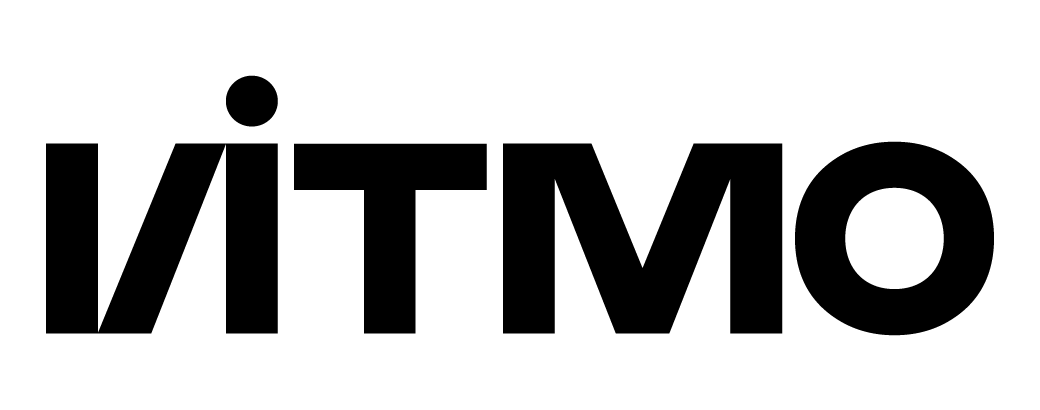
\includegraphics[scale=0.2]{../../lib/img/itmo.png}
    \end{center}

    \vspace{4cm}

    \begin{center}
      \large \textbf{Вариант \textnumero \commandkey{variant}}\\
      \textbf{Лабораторная работа \textnumero \commandkey{labn}}\\
      по дисциплине\\
      \textbf{\commandkey{discipline}}
    \end{center}

    \vspace*{\fill}

    \begin{flushright}
      Выполнил Студент группы \commandkey{group}\\
      \textbf{\commandkey{student}}\\
      Преподаватель: \\
      \textbf{\commandkey{teacher}}\\
    \end{flushright}

    \vspace{1cm}

    \begin{center}
      г. Санкт-Петербург\\
      \commandkey{year}г.
    \end{center}

    \thispagestyle{empty}
  \end{titlepage}
}



\begin{document}

\itmo[
  variant=74273.77,
  labn=7,
  discipline=Программирование,
  group=P3115,
  student=Владимир Мацюк,
  teacher=Кустарев Иван Павлович,
  year=2023,
  logo=../../../lib/img/itmo.png
]

\section*{Задание}

Доработать программу из лабораторной работы №6 следующим образом:

\begin{itemize}
  \item Организовать хранение коллекции в реляционной СУБД (PostgresQL). Убрать хранение коллекции в файле.
  \item Для генерации поля id использовать средства базы данных (sequence).
  \item Обновлять состояние коллекции в памяти только при успешном добавлении объекта в БД
  \item Все команды получения данных должны работать с коллекцией в памяти, а не в БД
  \item Организовать возможность регистрации и авторизации пользователей. У пользователя есть возможность указать пароль.
  \item Пароли при хранении хэшировать алгоритмом SHA-256
  \item Запретить выполнение команд не авторизованным пользователям.
  \item При хранении объектов сохранять информацию о пользователе, который создал этот объект.
  \item Пользователи должны иметь возможность просмотра всех объектов коллекции, но модифицировать могут только принадлежащие им.
  \item Для идентификации пользователя отправлять логин и пароль с каждым запросом.
\end{itemize}

Необходимо реализовать многопоточную обработку запросов.

\begin{itemize}
  \item Для многопоточного чтения запросов использовать Fixed thread pool
  \item Для многопотчной обработки полученного запроса использовать создание нового потока (java.lang.Thread)
  \item Для многопоточной отправки ответа использовать создание нового потока (java.lang.Thread)
  \item Для синхронизации доступа к коллекции использовать синхронизацию чтения и записи с помощью java.util.concurrent.locks.ReentrantLock
\end{itemize}

\section*{Порядок выполнения работы:}

\begin{itemize}
  \item В качестве базы данных использовать PostgreSQL.
  \item Для подключения к БД на кафедральном сервере использовать хост pg, имя базы данных - studs, имя пользователя/пароль совпадают с таковыми для подключения к серверу.
\end{itemize}

\section*{Отчёт по работе должен содержать:}

\begin{itemize}
  \item Текст задания.
  \item Диаграмма классов разработанной программы.
  \item Исходный код программы.
  \item Выводы по работе.
\end{itemize}

\section*{Диаграмма классов}

\begin{center}
  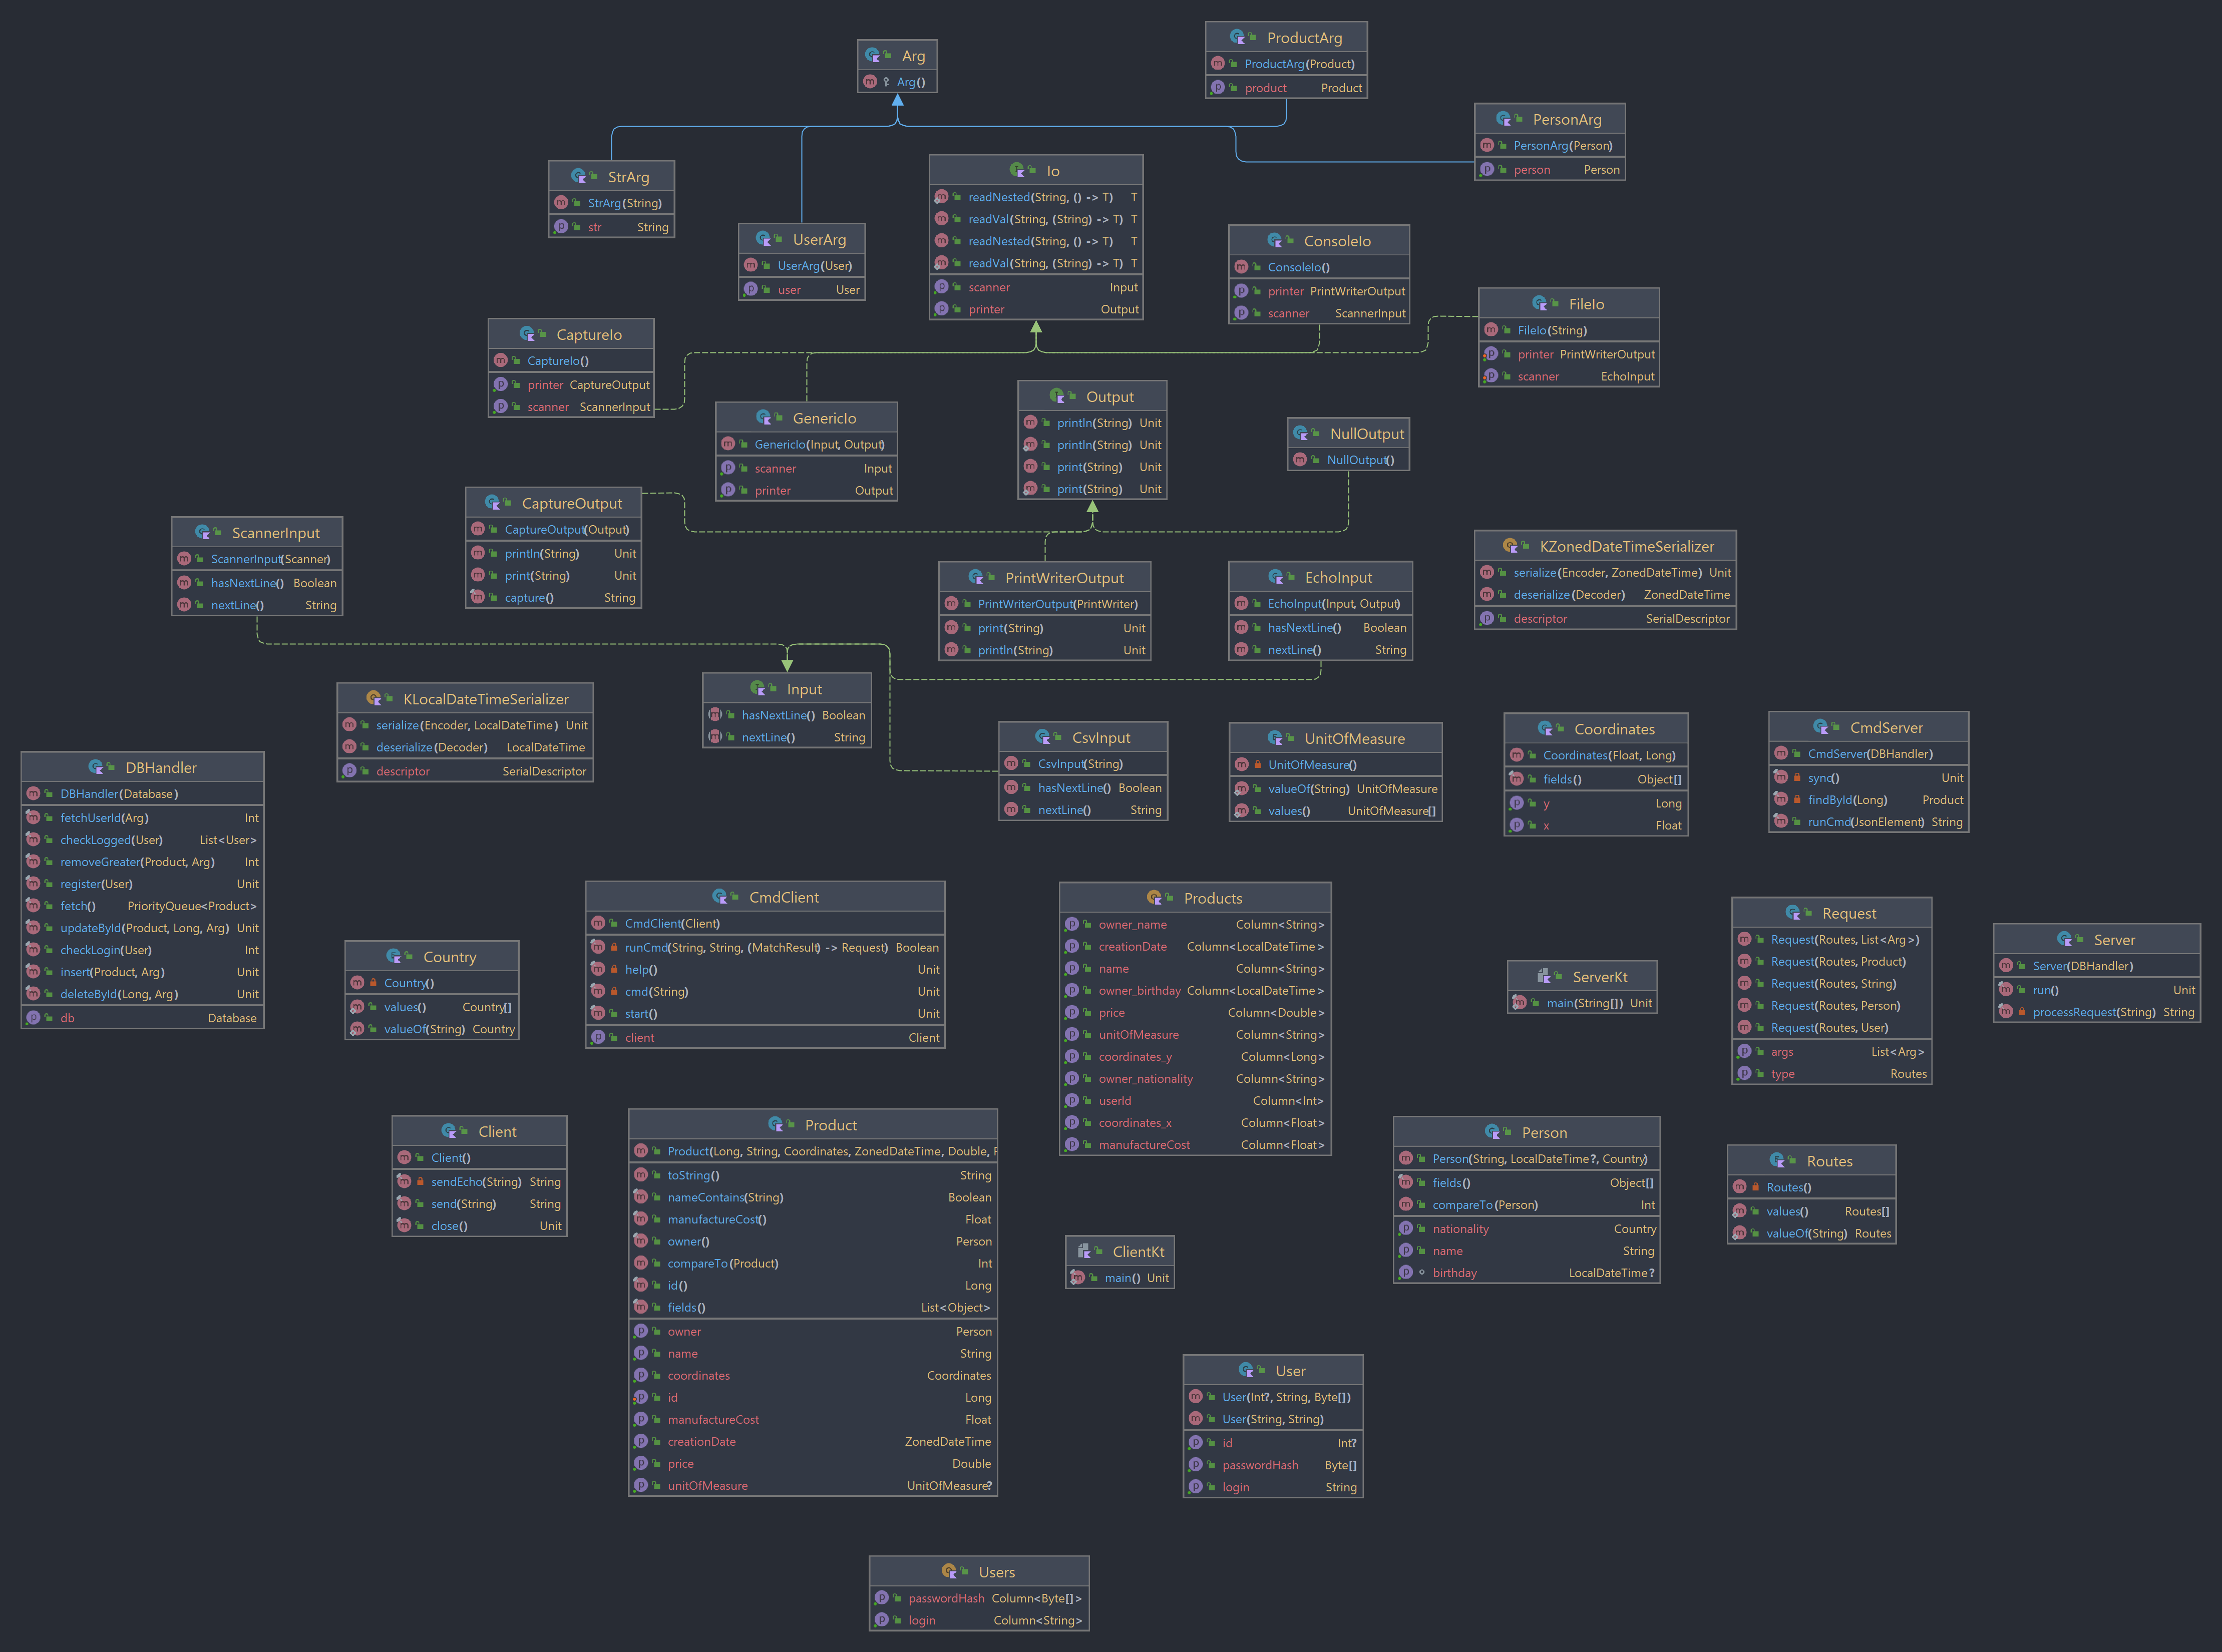
\includegraphics[scale=0.10]{diagram.png}
\end{center}

\section*{Исходный код}
\url{https://github.com/Wgmlgz/itmo2/tree/main/l7}

\section*{Вывод}
Во время выполнения работы я глубже ознакомился с ООП на языке java.
\end{document}
